\chapter{Planning Clásico}
\label{ch:lit_rev}

En este capítulo se detallaran una serie de definiciones teóricas, necesarias
para comprender el enfoque de esta tesis y sobre que parte de este campo
aplicaremos técnicas de aprendizaje automático. Partiendo desde el área de
\emph{planning}, detallando más concretamente que son los estados y acciones,
representación STRIPS de un problema, el lenguaje PDDL, el proceso de
\emph{grounding}, la complejidad de encontrar un plan que resuelva la tarea, y
la necesidad de tomar ventaja de planes relajados.

\section{¿Qué se entiende por planning?}

Durante nuestras actividades de la vida cotidiana, siempre estamos actuando y
anticipando el resultado de nuestras decisiones, aún si no estamos completamente
conciente de ello, o explícitamente planeando que hacer antes de realizar una
acción. No obstante, una tarea que abarque objetivos nuevos y complejos requiere
deliberación al consistir de acciones que uno no esta acostumbrado, tareas de
alto riesgo, o cooperación con alguien más.

\emph{Automated Planning} es el area de la inteligencia artificial que estudia
la deliberación de los procesos computacionales. Su objetivo es facilitar la
tarea de planificación por medio del razonamiento sobre representaciones
abstractas y formales del dominio, configuración inicial, combinación de
acciones, y objetivos a ser satisfacidos. El modelo conceptual del dominio en el
cual las acciones son ejecutadas es llamado \emph{dominio de planning}, y los
requerimientos inicial y final son denominados \emph{estado inicial} y
\emph{meta}. Estas 3 componentes definen un \emph{tarea de planning} cuyo
objetivo es encontrar alguna combinación de acciones que determinen un
\emph{plan}.

Algunos ejemplos de esto son la navegación de un robot, donde una acción altera
su posición siendo necesarias aquellas que lo lleven de una habitación a otra;
en el caso de un micro-procesador, una instrucción puede pensarse como una
acción que cambia el valor de sus registros y se busca que instrucciones son
necesarias para ejecutar un programa; un servicio web de vuelos de avion que
reciba un mensaje de reservación por un vuelo, siendo una acción que cambia su
estado, siempre y cuando no se sobrepase el número de reservaciones máximo a
partir de una cantidad inicial disponible. \citep{Sandewall-2008-HandbookOK}

\section{Estados y acciones}

Un mundo o estado  posible de una tarea de \emph{planning} se representa a
partir de un conjunto de símbolos proposicionales que modelan un aspecto del
entorno. Por ejemplo, el símbolo proposicional $p$ puede modelar la situación
``el agente $a_1$ se encuentra en la ubicación $l_1$``. Aquellos símbolos  que
no están mencionados en un estado, se asumen como no válidos en dicho mundo. De
esta manera, si se tienen los símbolos proposicionales $p,q,r$, $\{p, q\}$
representa el estado en el que vale $p$ y $q$ pero no $r$.

Las acciones son representadas en términos de una precondición y un efecto. La
precondición es una fórmula proposicional que representa la condición necesaria
para que la acción pueda ser llevada a cabo. Mientras que el efecto es una
fórmula que determina los cambios que produce la ejecución de la acción sobre el
entorno. Por ejemplo, consideremos la siguiente acción $A$:
\begin{align*}
    & Action : A \\
    & pre : p \land \neg r \\
    & eff : \neg p \land q
\end{align*}

$A$ no es aplicable en el estado $\{p, r\}$, ya que, no se cumple su
precondición, pero si en el estado $\{p\}$ transformandolo en el estado $\{q\}$.
Se puede interpretar las acciones como operadores de transformación de
estados en el que su ejecución genera que ciertos símbolos proposicionales
empiecen a valer o no según si estos ocurren positivamente o negativamente en el
efecto de la acción.

El tipo de fórmula que se permite en la precondición y en el efecto de las
acciones determina el tipo de la tarea de \emph{planning}. En particular, se
utilizaron tareas de \emph{planning} STRIPS durante el desarrolo de esta tesis.

\section{Tareas STRIPS}

El tipo de una tarea de \emph{planning} está dada por la lógica de las formulas
que ocurren en las acciones y en la meta. En STRIPS, las fórmulas son
conjunciones de literales, es decir, de la forma $\bigwedge_i l_i$ con $l_i$
un símbolo proposicional o su negación.

\begin{mydef}
    Una fórmula STRIPS es una fórmula $\phi$ tal que $\phi$ está en forma 1-CNF.
    Una acción $a$ es del tipo STRIPS si su precondición y su efecto son fórmulas
    STRIPS.
\end{mydef}

Una forma más conveniente de trabajar sobre esta representación es utilizando
únicamente conjuntos de símbolos proposicionales. Vimos que en el caso de los
estados, solo se mantienen aquellos que son válidos en el mundo, es decir, los
literales positivos. De manera similar, ocurre con la precondición de una
acción. Sin embargo, en el caso de su efecto se mantienen dos conjuntos, uno
con los símbolos proposicionales positivos, y otro con los negativos.

Por ejemplo, la acción $A$ que describimos anteriormente puede verse
de la siguiente forma:
\begin{align*}
    & Action : A \\
    & pre : \{ p \}\\
    & add : \{ q \}\\
    & del : \{ p \}
\end{align*}

La interpretación de $A$ es similar a la que se dió anteriormente, la
precondición contiene los símbolos proposicionales necesarios para que $A$ sea
aplicable en un mundo. Mientras que $add$ y $del$ son los conjuntos de símbolos
proposicionales que agrega y elimina la acción producto de su ejecución.

Esta nueva representación permite abstraer fórmulas y operadores
proposicionales, lo cual ayudará para introducir de manera más natural algunas
técnicas del área.

\begin{mydef}
    Una tarea de planning STRIPS es una 4-upla $\Pi = (F, A, I, G)$ donde $F$ es
    un conjunto finito de símbolos proposicionales denominados facts, $A$ es un
    conjunto finito de acciones STRIPS, $I \subseteq F$ el estado inicial, $G
    \subseteq F$ el estado final.
\end{mydef}

\begin{mydef}
    Sea $\Pi = (F, A, I, G)$ una tarea STRIPS.
    
    \begin{itemize}
        \item Un estado $s \subseteq F$ es un conjunto de facts. Diremos que un
        símbolo proposicional $p \in F$ vale en un estado $s$ sii $p \in s$.
        
        \item Una acción STRIPS es una 3-upla $a = (pre, add, del)$, tal que,
        $pre, add,$ y $del$ son subconjuntos de F, y los denotaremos como $pre(a)$,
        $add(a)$, y $del(a)$ respectivamente.

        \item Una acción $a$ es aplicable en un estado $s$ si $pre(a) \subseteq
        s$, en tal caso, el estado resultante es $s' = (s - del(a)) \cup
        add(a)$. Escribimos $s \xrightarrow{a} s'$ para la transición de $s$ a
        $s'$ vía $a$. Para una secuencia de acciones $\vec{a}$, escribimos $s
        \xrightarrow{\vec{a}} t$ si estos pueden ser iterativamente aplicados a
        $s$, resultando en $t$.

        \item Un plan para $\Pi$ es una secuencia $\vec{a}$ con $I
        \xrightarrow{\vec{a}} s_G$ si $G \subseteq s_G$.
        
        \item Una tarea $\Pi$ es satisfacible si un plan para $\Pi$ existe. El
        plan es denominado óptimo si es el que tiene longitud más corta de entre
        todos los planes para $\Pi$.
    \end{itemize}
\end{mydef}

Para ejemplificar estas definiciones consideremos el problema de la Figura
\ref{fig:agent_example} Tenemos único agente $a_1$ que se encuentra inicialmente
en la posición $l_1$ marcada en azúl y desea ir hacia la ubicación $l_4$ en
rojo. Los enlaces de la figura indican los posibles movimientos dentro del mapa.
La tarea STRIPS en este caso estaría dada por:

\begin{align*}
    F = \{&at(a_1, l_1), at(a_1, l_2), at(a_1, l_3), at(a_1, l_4)\} \\
    A = \{&move(a_1, l_1, l_2), move(a_1, l_2, l_1), \\
    & move(a_1, l_1, l_3), move(a_1, l_3, l_1),\\
    & move(a_1, l_3, l_4), move(a_1, l_4, l_3)\} \\
    I = \{&at(a_1, l_1)\} \\
    G = \{&at(a_1, l_4)\}
\end{align*}

Para cada agente $x$ y ubicaciones $l, l'$ se tiene que $move(x, l, l') =
({at(a, l)}, {at(a, l')}, {at(a, l)})$. Un posible plan de la tarea podría ser
la secuencia $\vec{a} = move(a_1, l_1, l_3)move(a_1, l_3, l_4)$.

\begin{figure}
    \centering
    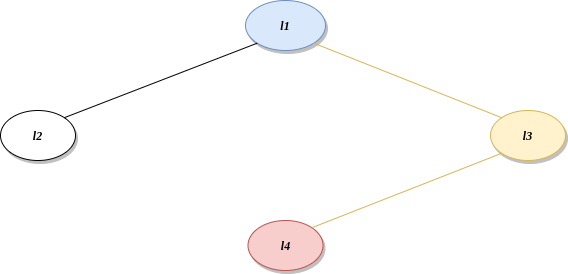
\includegraphics[scale=0.5]{figures/agent_example.png}
    \caption{Ejemplo del problema del agente. Su posición inicial es la ubicación
             $l1$ en azúl queriendo llegar a la posición $l4$ marcada con rojo.}
    \label{fig:agent_example}
\end{figure}


\section{Representaciones STRIPS}

Un dato de entrada necesario para cualquier algoritmo de planificación es una
descripción del problema a ser resuelto. En la práctica, es usualmente imposible
incluir una explicita enumeración de todos los estados y transiciones que se
pueden realizar en el dominio a partir de una tarea STRIPS. Por lo tanto, es
necesario una representación que permita computarlas dinámicamente.

Consideremos el problema del ejemplo anterior donde se tiene el agente $a_1$
pero esta vez $n$ ubicaciones. Para este caso, se va a necesitar $n$ símbolos
proposicionales $p_i$ tal que representen la acción ``El agente $a_1$ está en la
ubicación $i$``. Si en lugar de un solo agente hubiesen una cantidad $m$ de
ellos. Se necesitarian $n \times m$ símbolos para modelar esta caracteristica de
la tarea. Una forma más compacta de representar esta propiedad es por medio de
un predicado de la forma $at(x, l)$ donde $x$ denota a un agente, y $l$ su
ubicación, siendo mucho más flexible debido a su naturaleza esquematica.

De manera similar, si se quisiera modelar una acción de cambio de posición,
haría falta describir una por cada agente y par de ubicaciones obteniendo un
total de $m \times n \times n$ instancias. Una mejor alternativa es representar
esta transformación por medio de un esquema de acción de la forma $move(x, l,
l')$ donde $x$ representa al agente, $l$ la ubicación actual, y $l'$ la ubicación
a la cual moverse.

De esta forma resulta más adecuado para la especificación utilizar predicados y
esquemas de acción en lugar de símbolos proposicionales. Esto lleva a las
siguientes definiciones:

\begin{mydef}
    Una especificación de una tarea STRIPS es una 6-upla $(\mathcal{P},
    \mathcal{A}, \Sigma^{C}, \Sigma^{O}, I, G)$  donde $\mathcal{P}$ es un
    conjunto de predicados, $\mathcal{A}$ es un conjunto de esquemas de acción,
    $\Sigma^{C}$ es un conjunto de constantes, $\Sigma^{O}$ es un conjunto de
    objetos no constantes, $I$ es el estado inicial, y $G$ es la meta.
\end{mydef}

\begin{mydef}
    Sea $(\mathcal{P}, \mathcal{A}, \Sigma^{C}, \Sigma^{O}, I, G)$ una
    especificación de una tarea STRIPS.

    \begin{itemize}
        \item Un esquema de acción es una 3-upla $a[X] = (pre(a), add(a),
        del(a))$ donde cada elemento es subconjunto de $\mathcal{P}$, y $X$ es el
        conjunto de variables que ocurren en $pre(a) \cup add(a) \cup del(a)$ y
        que son parte de $\Sigma^{O}$.
        \item Un predicado es un símbolo atómico de $\mathcal{P}$ de la forma
        $p[X]$ con $X$ un conjunto de variables que ocurren en su interfaz y
        que son parte de $\Sigma^{O}$.
    \end{itemize}
\end{mydef}

Para la tarea STRIPS del problema del agente se tiene que su especificación está
dada por

\begin{align*}
    \mathcal{P} = \{&at(x, l)\} \\
    \mathcal{A} = \{&move(x, l, l')\} \\
    \Sigma^{C} = \{&a_1, l_1, l_2, l_3, l_4\} \\
    \Sigma^{O} = \{&x, l, l'\} \\
    I = \{&at(a_1, l_1)\} \\
    G = \{&at(a_1, l_4)\}
\end{align*}

Una diferencia importante es que ahora $move$ es un esquema de acción dado por:

\begin{align*}
    move(x, l, l') &= (pre(move), add(move), del(move)) \\
                   &= (\{at(x, l)\}, \{at(x, l')\},\{at(x, l)\})
\end{align*}

Por otro lado, las variables y objetos que se utilizaban para expresar todas las
proposiciones lógicas se hicieron parte de la especificación logrando expresar
predicados y acciones de manera esquematica.

\section{El lenguaje PDDL}

Para especificar una tarea de planning a una computadora se necesita definir un
lenguaje que permita al usuario definir cada una de sus componentes. Para dar
respuesta a esta necesidad surge el \emph{Planning Domain Specification
Language} (PDDL), Propuesta por Drew Mc Dermott para la competencia de planning
AIPS-98 \citep{McDermott1998} siendo la heramienta más conocida y usada dentro
de la comunidad de planning.

Una especificación en PDDL consiste de dos archivos, la definición del dominio,
donde se aclaran los predicados y esquemas de acción disponibles; y la
definición de la tarea donde se mencionan los objetos concretos a modelar, el
estado inicial, y la meta. Esta separación resulta importante ya que diferentes
tareas de un mismo dominio comparten una estructura común.

Los Listing \ref{lst:agent-domain} y \ref{lst:agent-task} muestran los archivos
de dominio y tarea del ejemplo del agente escritas en PDDL.

\begin{lstlisting}[
    float=!htb,
    caption={Dominio Agent en PDDL.},
    label={lst:agent-domain},
    language=PDDL]
  (
    define (domain AGENT-DOMAIN)

    (:requirements :strips :typing)

    (:types AGENT LOCATION)

    (:predicates (at ?x - AGENT ?y - LOCATION))

    (:action move
        :parameters (?x - AGENT ?s - LOCATION ?d - LOCATION)
        :precondition (and (at ?x ?s))
        :effect (and (not (at ?x ?s)) (at ?x ?d))
    )
  )
\end{lstlisting}

\begin{lstlisting}[
    float=!htb,
    caption={Ejemplo de una tarea del dominio Agent en PDDL.},
    label={lst:agent-task},
    language=PDDL]

  (
    define (problem AGENT-TASK)

    (:domain AGENT-DOMAIN)

    (:objects a1 - AGENT l1 l2 l3 l4 - LOCATION)

    (:init at(a1, l1))
    
    (:goal (and at(a1, l4)))
  )
\end{lstlisting}

\section{Relajación por deletes}

El problema de decidir si una tarea de planning STRIPS tiene un plan es
PSPACE-completo, lo cual lo hace intratable para problemas complejos
\citep{Nau-Ghallab-Malik-Traverso-2004}. Sin embargo, en ocasiones se suelen
realizar simplificaciones para obtener uno nuevo, a priori más sencillo de
resolver, que aporte información para lidiar con el original. En particular, la
\emph{relajación por deletes} es una simplificación de la tarea que consiste en
eliminar los efectos negativos de una acción, es decir, su lista $del$. Esta
relajación es ampliamente utilizada en planning y su importancia subyace en la
siguiente propiedad: en la \emph{relajación por deletes} si un \emph{fact} se
vuelve válido, entonces permanecerá válido para siempre. Por ejemplo, en el
problema del agente, si este se desplazó por varias ubicaciones, tendriamos que
se encuentra en más de un lugar al mismo tiempo ya que la proposición que
indicaba su ubicación anterior no puede ser borrada.

Claramente es una modelización no realista, no obstante, encontrar un plan en una
tarea relajada puede ser computada en tiempo polinomial, y en la práctica
resulta ser una buena aproximación a un plan del problema inicial.

\begin{mydef}
    Sea $\Pi = (F, A, I, G)$ una tarea STRIPS.
    \begin{itemize}
        \item Sea $a \in A$, definimos a la acción relajada por delete $a^{+}$
        dada por $pre(a^{+}) = pre(a)$, $add(a^{+}) = add(a)$, y $del(a^{+}) =
        \emptyset$.

        \item Denotaremos con $A^{+} = \{a^{+} : a \in A\}$ al conjunto de
        acciones relajadas por delete.

        \item Para una secuencia de acciónes $\vec{a}$ denotaremos con
        $\vec{a}^{+}$ a la secuencia de acciones relajadas por delete.

        \item Denotaremos con $\Pi^{+} = (F, A^{+}, I, G)$ a la tarea STRIPS
        relajada por deletes.

        \item Un plan relajado para $\Pi$ es un plan para $\Pi^{+}$.
    \end{itemize}
\end{mydef}

\section{Proceso de grounding}

Dada una especificación de una tarea STRIPS $(\mathcal{P}, \mathcal{A},
\Sigma^{C}, \Sigma^{O}, I, G)$ se puede obtener su correspondiente tarea $\Pi =
(F, A, I, G)$ recolectando todas las instancias posibles de predicados en
$\mathcal{P}$ y esquemas de acción de $\mathcal{A}$ con objetos de $\Sigma^{C}$.
Es decir, $F$ contiene un \emph{fact} por cada posible asignación de objetos a
los argumentos de cada predicado $P[X] \in \mathcal{P}$, y $A$ contiene una
acción por cada posible asignación de objetos a los argumentos de cada esquema
de acción $a[X] \in \mathcal{A}$. Este proceso se conoce como \emph{Grounding
Cartesiano}.

No obstante, en la práctica los planificadores no enumeran todos las posibles
acciones y proposiciones, si no aquellas que son alcanzables relajadamente desde
el estado inicial. Esto viene de la premisa de que un plan de una tarea también
es solución de su contraparte relajada, garantizando de esta manera que
cualquier otra solución se puede formar con aquellas instanceas groundeadas
relajadamente.

Este proceso de grounding es el implementado por el planificador \emph{Fast
Downward} \citep{Helmert-2011} y es sobre el cual se adaptará para utilizar
técnicas de aprendizaje automático.

\begin{mydef}
    Sea $\Pi = (F, A, I, G)$ una tarea STRIPS.    
    \begin{itemize}
        \item Un estado $s \subseteq F$ es alcanzable en $\Pi$ si existe una
        secuencia $\vec{a}$ de acciones tal que $I \xrightarrow{\vec{a}} s$.
    
        \item Un proposición $p \in F$ es alcanzable en $\Pi$ si existe un estado
        $s$ alcanzable en $\Pi$ tal que $p \in s$.

        \item Una acción $a \in A$ es alcanzable en $\Pi$ si existe una estado $s$
        alcanzable en $\Pi$ tal que $a$ es aplicable en $s$.

        \item Un proposición $p \in F$ es alcanzable relajadamente en $\Pi$ si
        $p$ es alcanzable en $\Pi^{+}$.

        \item Una acción $a \in A$ es alcanzable relajadamente en $\Pi$ si
        $a^{+}$ es alcanzable en $\Pi^{+}$.
    \end{itemize}
\end{mydef}


\begin{algorithm}
    \caption{Grounding por alcanzabilidad
    relajada}\label{alg:grounding_delete_relaxed}
    \begin{algorithmic}
    \Require Especificación de una tarea STRIPS $(\mathcal{P}, \mathcal{A},
    \Sigma^{C}, \Sigma^{O}, I, G)$
    \Ensure Tarea STRIPS $(F, A, I, G)$ 
    \State $q \gets I$
    \State $F \gets \emptyset$
    \State $A \gets \emptyset$
    \While{$ \lnot (q.empty() \lor G \subseteq F)$}
    \State $e \gets q.pop()$
    \If{e is fact}
        \State $F \gets F \cup \{e\}$
        \For{$a \notin A \land pre(a) \subseteq F$}
            \State $q.insert(a)$
        \EndFor
    \Else
        \State $A \gets A \cup \{e\}$
        \For{$f \notin F \land f \in add(e)$}
            \State $q.insert(f)$
        \EndFor
    \EndIf
    \EndWhile
    \State \Return $(F, A, I, G)$
    \end{algorithmic}
\end{algorithm}

El algoritmo \ref{alg:grounding_delete_relaxed} implementado por Fast Downward
parte de una cola $q$ que almacena todos los símbolos proposicionales del estado
inicial. A partir de allí, se remueve elemento a elemento de $q$ consultando si
es un hecho o una acción.

En el caso de encontrarse con un hecho, se lo instancia y se agregan a $q$ todas
las acciones aplicables (aún no procesadas) a partir de las proposiciones
groundeadas hasta el momento. Caso contrario, se obtiene una acción que también
se instancia y se agregan a $q$ todas las proposiciones (aún no procesadas) que
ocurren positivamente en su efecto, es decir, su lista $add$.

Este procedimiento se repite hasta que la cola se encuentre vacía o hasta que la
tarea STRIPS resultante sea satisfacible relajadamente a partir de las
instancias hasta el momento, esto es, si $G \subseteq F$. Un detalle a notar
es que si la cola se encuentra vacía, entonces se obtiene el resultado de
Grounding Cartesiano.

\section{Grounding heurístico}

Mencionamos que un plan de una tarea es también un plan relajado de la misma.
Sin embargo, el reciproco no se cumple. Es más, un hecho o una acción que es
relajadamente alcanzable, puede no ser alcanzable en la tarea original o ser
irrelevante al no pertenecer a ningun plan que la resuelva. Es justamente esta
pérdida de información la que origina que computar en el mundo relajado sea
polinomial. Es aquí donde surge el foco de este trabajo donde se intentará
predecir cual de estos hechos y acciones son verdaderamente relevantes para
alcanzar la meta, priorizando su instanciación por sobre el resto.

El algoritmo de grounding heurístico que presentaremos es el mismo que se
desarrolló en \citep{Gnad_Torralba_Dominguez_Areces_Bustos_2019} y está basado
en el que se mostró en la sección anterior. Las principales diferencias son el
criterio de parada, donde se procesan no más de $N$ acciones, y el orden en que
lo hacen, según su nivel de relevancia. Debido a que el algoritmo puede
terminar antes de que la cola se vacíe, se está obligado a procesar la totalidad
de los facts existentes antes de considerar una siguiente acción. Esto garantiza
que todos los facts que se encuentran en los efectos de las acciones ya
procesadas están en $F$ siendo el algoritmo \emph{fact consistente}.

\begin{mydef}
    Sean $F$ y $A$ el conjunto de facts y acciones retornados por un algoritmo
    de grounding. Decimos que este es fact consistente si para todo $a \in A$ se
    cumple que, si $p \in pre(a) \cup add(a) \cup del(a)$ entonces $p \in F$.
\end{mydef}

\begin{algorithm}
    \caption{Grounding heurístico}\label{alg:grounding-heuristico}
    \begin{algorithmic}
    \Require Especificación de una tarea STRIPS $(\mathcal{P}, \mathcal{A},
    \Sigma^{C}, \Sigma^{O}, I, G)$
    \Ensure Tarea STRIPS $(F, A, I, G)$ 
    \State $q \gets I$
    \State $F \gets \emptyset$
    \State $A \gets \emptyset$
    \While{$ \lnot (q.empty() \lor G \subseteq F) \land |A| \leq N$}    
    \If{$q.containsFact()$}
        \State $f \gets q.popFact()$
        \State $F \gets F \cup \{f\}$
        \For{$a \notin A \land pre(a) \subseteq F$}
            \State $q.insert(a)$
        \EndFor
    \Else
        \State $a \gets q.popHighPriorityAction()$
        \State $A \gets A \cup \{a\}$
        \For{$f \notin F \land f \in add(a)$}
            \State $q.insert(f)$
        \EndFor
    \EndIf
    \EndWhile
    \State \Return $(F, A, I, G)$
    \end{algorithmic}
\end{algorithm}

En grounding heurístico, el algoritmo puede detenerse mucho antes según el
parámetro $N$ que indica la cantidad de instancias que puede realizar el proceso
sin que los recursos de tiempo y memoria se vean comprometidos. Por lo general,
muchas de los problemas de planning requieren planes cortos del orden de a lo
sumo cientos de acciones en comparación a posiblemente millones de operadores
groundeados.

Es importante mencionar que este algoritmo es \emph{correcto}, si hallamos un
plan de la tarea obtenida por grounding heurístico, entonces ese mismo plan lo
es para la tarea obtenida por grounding total. No obstante, no es
\emph{completo}, una tarea obtenida por grounding heurístico tiene solución si y
sólo si las acciones correspondientes de al menos un plan (de la tarea obtenida
por grounding total) fueron procesadas.

Por último, algo a considerar es el remplazo de la cola del Algoritmo
\ref{alg:grounding-heuristico}, por una cola de prioridades que asigna a las
acciones un nivel de relevancia por la cual son ordenadas. La relevancia de una
acción está directamente relacionada con la probabilidad de que esta pertenezca
a un plan de la tarea. Notar que una estimación ideal sería una probabilidad de
1 para las acciones que ocurren en algún plan de la tarea y 0 para las
restantes. Pero computar esto es a la vez tan difı́cil como obtener una solución
y sabemos que es PSPACE-completo. Es por eso que para estimar la relevancia se
utilizaron técnicas de aprendizaje automático y serán el foco del siguiente
capítulo.
